\documentclass[11pt,a4paper]{article}

% ===================== Paquetes =====================
\usepackage[utf8]{inputenc}
\usepackage[T1]{fontenc}
\usepackage[margin=2.3cm]{geometry}
\usepackage{booktabs}
\usepackage{longtable}
\usepackage{array}
\usepackage{tabularx}
\usepackage{graphicx}
\usepackage{xcolor}
\usepackage{caption}
\usepackage{float}
\usepackage{pdflscape}
\usepackage{listings}
\usepackage{enumitem}
\usepackage[hidelinks]{hyperref}

\definecolor{codebg}{RGB}{245,245,245}
\lstset{
  basicstyle=\ttfamily\footnotesize,
  backgroundcolor=\color{codebg},
  breaklines=true,
  frame=single,
  columns=fullflexible,
  keepspaces=true,
  showstringspaces=false
}
\newcommand{\ip}[1]{\texttt{#1}}
\captionsetup{font=small,labelfont=bf}

% ===================== Portada =====================
\title{\textbf{Tarea Individual --- Path Discovery}\\[0.3em]
\large Comparación de tráfico entre RIPE Atlas y Scamper}
% EDITABLE: ajuste su nombre si corresponde
\author{Laura Romero \\ \texttt{laura.romero@mail.udp.cl}}
\date{Octubre 2026}

\begin{document}
\maketitle

\begin{abstract}
\noindent Este informe caracteriza la infraestructura de Internet utilizada por una conexión de
Banda Ancha Fija (BAF) del ISP \textbf{Entel Chile (AS27651)}, mediante técnicas de
\emph{path discovery}. Se comparan dos herramientas de medición activa: \textbf{scamper}
(versión 20260902) ejecutado localmente y la plataforma \textbf{RIPE Atlas} (sonda por software
ID~1018349). Se miden rutas hacia tres sondas RIPE representativas: Valparaíso
(\ip{138.204.228.2}, mayor velocidad mundial), La Habana (\ip{200.14.48.134}, peor velocidad
mundial) y Rusia (\ip{37.79.153.66}, mayor censura reciente). Se analizan los seis métodos de
traceroute de scamper, los cinco modos de \texttt{tracelb}, los tres protocolos de RIPE, el
tráfico generado a nivel de capa de transporte, las reglas de filtrado detectadas, la
asimetría de ruteo ida/vuelta y, finalmente, se publican tres grafos de ruta en NDEx.
\end{abstract}

\tableofcontents
\clearpage

% ======================================================================
\section{Introducción}
% ======================================================================
El \emph{path discovery} o descubrimiento de rutas es el proceso de inferir, a partir de
mediciones de red activas, la secuencia de dispositivos (routers) que atraviesa un paquete
desde un origen hasta un destino en Internet. Su herramienta clásica es el \emph{traceroute},
cuyo principio de funcionamiento se apoya en un campo de la cabecera IP: el \emph{Time To Live}
(TTL). Cada router que reenvía un paquete decrementa el TTL en una unidad; cuando éste llega a
cero, el router descarta el paquete y devuelve al origen un mensaje de error ICMP de tipo~11
(\emph{Time Exceeded}). Enviando sondas con TTL creciente (1, 2, 3, \dots) y observando qué
dirección IP origina cada \emph{Time Exceeded}, se reconstruye salto a salto la ruta. El último
salto se confirma cuando el propio destino responde (con un \emph{Echo Reply}, un
\emph{Port Unreachable} o un \emph{RST}, según la técnica empleada).

El objetivo de este trabajo es caracterizar la infraestructura de Internet que utiliza una
conexión de Banda Ancha Fija (BAF) real, contrastando dos enfoques complementarios de medición:
\textbf{scamper}, una herramienta de medición activa desarrollada por CAIDA que se ejecuta
localmente sobre el enlace del usuario, y \textbf{RIPE Atlas}, una plataforma global de sondas
distribuidas que permite lanzar mediciones desde miles de puntos de observación. Mientras
scamper ofrece un control fino del tipo de sonda enviada (seis métodos de traceroute más cinco
modos de descubrimiento de balanceo de carga), RIPE Atlas aporta la capacidad de medir
\emph{también en sentido inverso}, es decir, desde el destino hacia el origen, lo que resulta
indispensable para evidenciar la asimetría del ruteo en Internet.

A lo largo del informe se sigue un recorrido progresivo: primero se caracteriza el punto de
observación (ISP, sistema autónomo y prefijo); luego se descubre la ruta con scamper y se
analiza en detalle el tráfico generado por cada técnica; a continuación se replica el proceso
con RIPE Atlas, incorporando la correspondencia de cada salto con su sistema autónomo; después
se mide la ruta de vuelta y se contrasta con la de ida; y finalmente se sintetiza el
conocimiento obtenido en tres grafos de ruta publicados en el repositorio NDEx. En cada etapa se
documenta no sólo el resultado, sino el procedimiento que lo produjo y la interpretación técnica
de lo observado, con especial atención a las reglas de filtrado que dificultan el reconocimiento
de la red y a cómo un auditor podría sortearlas.

% ======================================================================
\section{Caracterización del entorno (BAF)}
% ======================================================================
Todo ejercicio de \emph{path discovery} comienza por situar el punto de observación: no es lo
mismo medir desde una red académica que desde un acceso residencial, porque la posición en la
jerarquía de Internet condiciona por completo las rutas que se verán. Por ello el primer paso es
identificar el proveedor (ISP), el sistema autónomo (AS) al que pertenece la IP pública y el
prefijo que dicho AS anuncia por BGP. Para categorizar los resultados se identifica el ISP y el
prefijo de la IP pública, según la información del AS (sitio \url{https://bgp.he.net}).

\begin{table}[H]
\centering
\begin{tabularx}{\textwidth}{l X}
\toprule
\textbf{Dato} & \textbf{Valor} \\
\midrule
IP pública & \ip{186.10.176.77} (rDNS: \texttt{z276.entelchile.net}) \\
ISP & ENTEL CHILE S.A. \\
ASN & \textbf{AS27651} (registrado en LACNIC, 2002-12-04) \\
Prefijo asignado (LACNIC \texttt{inetnum}) & \ip{186.10.128.0/18} \\
Prefijo anunciado por BGP (bgp.he.net) & \textbf{\ip{186.10.176.0/24}} \\
País & CL (Chile) \\
\bottomrule
\end{tabularx}
\caption{Identificación de la conexión BAF. El prefijo anunciado por BGP (\ip{/24}) es más
específico que el bloque asignado (\ip{/18}): Entel desagrega el \ip{/18} para su publicación BGP.}
\end{table}

El dato más relevante de esta tabla es la distinción entre el \emph{prefijo asignado} y el
\emph{prefijo anunciado}. LACNIC, el registro regional, delegó a Entel el bloque
\ip{186.10.128.0/18} (16.384 direcciones). Sin embargo, en la tabla de ruteo global Entel no
anuncia ese bloque completo de forma monolítica, sino que lo \emph{desagrega} en prefijos más
específicos, entre ellos el \ip{186.10.176.0/24} al que pertenece nuestra IP. Esta práctica es
habitual en operadores grandes: permite hacer ingeniería de tráfico (dirigir distintos bloques
por distintos enlaces de salida) y acotar el impacto de eventuales secuestros de ruta. Para el
análisis posterior esto importa porque fija el \emph{origen} de todas las mediciones: cualquier
ruta descubierta nacerá dentro de AS27651 y lo abandonará por los puntos de interconexión que
Entel mantiene con sus proveedores de tránsito internacional.

\paragraph{IPs destino (sondas RIPE Atlas).}
\begin{table}[H]
\centering
\begin{tabular}{llll}
\toprule
\textbf{Representa} & \textbf{IP destino} & \textbf{ID RIPE} & \textbf{AS destino} \\
\midrule
Valparaíso (mayor velocidad) & \ip{138.204.228.2} & 31416 & AS61506 INSACOM (CL) \\
La Habana (peor velocidad) & \ip{200.14.48.134} & 12734 & AS27725 ETECSA (CU) \\
Rusia (mayor censura) & \ip{37.79.153.66} & 870 & AS12389 Rostelecom (RU) \\
\bottomrule
\end{tabular}
\caption{Destinos de medición y su sistema autónomo.}
\end{table}

\paragraph{Instalación de scamper 20260902.} Se compiló desde el código de CAIDA. Fue necesario
\texttt{--disable-scamper-privsep} para poder ejecutarlo con \emph{capabilities} (sin root):
la separación de privilegios requiere root real para hacer \texttt{chroot}/\texttt{setuid} a
\texttt{/var/empty}.
\begin{lstlisting}[language=bash]
curl -O https://www.caida.org/catalog/software/scamper/code/scamper-cvs-20260902.tar.gz
tar xzf scamper-cvs-20260902.tar.gz && cd scamper-cvs-20260902
./configure --disable-scamper-privsep && make -j4 && sudo make install && sudo ldconfig
sudo setcap cap_net_raw,cap_net_admin+ep /usr/local/bin/scamper
scamper -v   # -> scamper version 20260902
\end{lstlisting}

\paragraph{Nota metodológica (red de la VM).} El equipo de medición es una máquina virtual
VMware, y este detalle, lejos de ser anecdótico, condicionó la viabilidad de todo el experimento.
En la configuración inicial en modo \textbf{NAT}, las primeras trazas sólo mostraban el salto~1
(el \emph{gateway} virtual de VMware) seguido de una cadena interminable de asteriscos. La causa
es instructiva y constituye en sí misma un primer hallazgo de \emph{path discovery}: el
dispositivo NAT de VMware traduce las sondas salientes, pero \emph{no es capaz de correlacionar}
los mensajes ICMP \emph{Time-Exceeded} que generan los routers intermedios con la sesión NAT
original, de modo que los descarta silenciosamente. El resultado es una red artificialmente
``muda'' más allá del primer salto. La solución fue reconfigurar el adaptador de red en modo
\textbf{bridged}, con lo que la VM obtiene una dirección propia en la LAN física y los
\emph{Time-Exceeded} regresan directamente a ella sin pasar por la traducción. Tras el cambio, la
IP pública observada se mantuvo (\ip{186.10.176.77}), confirmando que seguíamos midiendo sobre el
mismo acceso de Entel, pero ahora con visibilidad completa de la ruta. Este episodio ilustra un
principio general: un \emph{middlebox} que no reenvía correctamente los errores ICMP puede ocultar
por completo la topología situada detrás de él.

% ======================================================================
\section{Path Discovery con Scamper}
% ======================================================================
Instalada y verificada la herramienta, el procedimiento consistió en lanzar, hacia cada uno de
los tres destinos, una traza con cada uno de los seis métodos de \texttt{scamper trace -P}:
\texttt{udp}, \texttt{icmp}, \texttt{udp-paris}, \texttt{icmp-paris}, \texttt{tcp} y
\texttt{tcp-ack}. La razón de probar seis variantes, y no una sola, es que cada técnica construye
la sonda de forma distinta y, por tanto, interactúa de manera diferente con los filtros de la
red: un nodo que descarta UDP puede responder a ICMP, y un balanceador de carga puede desviar
cada método por una rama física distinta. Conviene distinguir dos familias. Los métodos
\emph{clásicos} (\texttt{udp}, \texttt{icmp}, \texttt{tcp}) varían algún campo de la cabecera de
transporte entre sondas sucesivas --típicamente el puerto destino--, lo que altera la ``5-tupla''
que los routers con \emph{Equal-Cost Multi-Path} (ECMP) usan para repartir el tráfico; en
consecuencia, sondas de distinto TTL pueden tomar caminos paralelos distintos y producir rutas
inconsistentes con saltos fantasma. Los métodos \emph{Paris} (\texttt{udp-paris},
\texttt{icmp-paris}) nacieron precisamente para corregir ese artefacto: mantienen constante la
5-tupla (fijando puertos e identificadores) y codifican el número de secuencia de la sonda en un
campo que \emph{no} participa del \emph{hash} de balanceo --el \emph{checksum}--, de modo que
todas las sondas siguen un único camino coherente. Finalmente, \texttt{tcp} (SYN) y
\texttt{tcp-ack} emplean segmentos TCP para atravesar firewalls que sólo permiten tráfico web.

Para UDP/TCP se usó el puerto de sonda \ip{33435}. Cada medición se acompañó de una captura de
paquetes con \texttt{dumpcap}, de manera que a cada traza le corresponde un archivo \texttt{.warts}
(formato nativo de scamper), su conversión a texto y un \texttt{.pcap} analizable en Wireshark.

\begin{lstlisting}[language=bash]
dumpcap -i eth0 -q -f "host $ip or icmp" -w evidencia/pcap/${tag}.pcap &
scamper -O warts -o evidencia/warts/${tag}.warts -I "trace -P $m $ip"
sc_warts2text evidencia/warts/${tag}.warts
\end{lstlisting}

\subsection{Tabla 1 --- Rutas por método}

\begin{landscape}
\begin{table}[H]
\centering\scriptsize
\begin{tabular}{c|llllll}
\toprule
HOP & udp & icmp & udp-paris & icmp-paris & tcp & tcp-ack \\
\midrule
1 & 192.168.100.1 & 192.168.100.1 & 192.168.100.1 & 192.168.100.1 & 192.168.100.1 & 192.168.100.1 \\
2 & 100.83.128.1 & 100.83.128.1 & 100.83.128.1 & 100.83.128.1 & 100.83.128.1 & 100.83.128.1 \\
3 & 10.253.197.9 & 10.253.197.9 & 10.253.197.9 & 10.253.197.9 & 10.253.197.9 & 10.253.197.9 \\
4 & 10.253.197.10 & 10.253.197.10 & 10.253.197.10 & 10.253.197.10 & 10.253.197.10 & \textbf{138.204.228.2 [RST]} \\
5 & 10.253.196.97 & 10.253.196.97 & 10.253.196.97 & 10.253.196.97 & 10.253.196.97 & --- \\
6 & 192.168.8.193 & 192.168.8.193 & 192.168.8.193 & 192.168.8.193 & 192.168.8.193 & --- \\
7 & 45.68.16.129 & 45.68.16.129 & 10.100.154.1 & 45.68.16.129 & 45.68.16.129 & --- \\
8 & 10.100.154.1 & 10.100.154.1 & 138.204.228.164 & 10.100.154.1 & 10.100.154.1 & --- \\
9 & 138.204.228.164 & 138.204.228.164 & 138.204.228.162 & 138.204.228.164 & * & --- \\
10 & 138.204.228.162 & 138.204.228.162 & * & 138.204.228.162 & * & --- \\
11 & * & \textbf{138.204.228.2} & * & \textbf{138.204.228.2} & * & --- \\
12--15 & * & & * & & * & --- \\
\bottomrule
\end{tabular}
\caption{Tabla 1 --- Destino Valparaíso \ip{138.204.228.2}. Llegan al destino: ICMP e ICMP-Paris
(11 saltos). UDP/UDP-Paris/TCP no completan. TCP-ACK ``llega'' en el salto 4 con un RST falso
(ver §\ref{sec:filtro}).}
\end{table}

\begin{table}[H]
\centering\scriptsize
\begin{tabular}{c|llllll}
\toprule
HOP & udp & icmp & udp-paris & icmp-paris & tcp & tcp-ack \\
\midrule
1--6 & \multicolumn{6}{l}{\ip{192.168.100.1} $\to$ \ip{100.83.128.1} $\to$ \ip{10.253.197.9} $\to$ \ip{10.253.197.10} $\to$ \ip{10.253.196.97} $\to$ \ip{192.168.9.133}} \\
7 & * & 213.99.17.182 & 5.53.3.71 & * & * & \ip{200.14.48.134 [RST]} (hop 4) \\
8 & 5.53.5.41 & 5.53.5.41 & 213.140.35.110 & 5.53.5.41 & 5.53.5.41 & \\
9 & 213.140.35.110 & 213.140.35.86 & 193.251.143.67 & 213.140.35.86 & * & \\
10 & 193.251.143.67 & 193.251.143.67 & * & 193.251.143.67 & * & \\
13 & 200.0.16.62 & 200.0.16.62 & 200.0.16.21 & 200.0.16.62 & 200.0.16.62 & \\
14 & 200.0.16.21 & 200.0.16.21 & 200.0.16.29 & 200.0.16.21 & 200.0.16.21 & \\
15 & 200.0.16.25 & 200.0.16.29 & 200.0.16.29 & 200.0.16.29 & 200.0.16.29 & \\
18 & 200.14.48.178 & 200.14.48.178 & 200.14.48.178 & 200.14.48.178 & * & \\
19/20 & \textbf{200.14.48.134} & \textbf{200.14.48.134} & \textbf{200.14.48.134} & \textbf{200.14.48.134} & \textbf{200.14.48.134} & \\
\bottomrule
\end{tabular}
\caption{Tabla 1 --- Destino La Habana \ip{200.14.48.134} (resumida; saltos \ip{*} intermedios
omitidos). Aquí \textbf{todos} los métodos salvo TCP-ACK alcanzan el destino. UDP es el más
completo (20 saltos).}
\end{table}

\begin{table}[H]
\centering\scriptsize
\begin{tabular}{c|llllll}
\toprule
HOP & udp & icmp & udp-paris & icmp-paris & tcp & tcp-ack \\
\midrule
1--6 & \multicolumn{6}{l}{\ip{192.168.100.1} $\to$ \ip{100.83.128.1} $\to$ \ip{10.253.197.9} $\to$ \ip{10.253.197.10} $\to$ \ip{10.253.196.97} $\to$ \ip{192.168.9.133}} \\
7 & 213.99.17.182 & 213.99.17.182 & 5.53.5.41 & 213.99.17.182 & 213.99.17.182 & \ip{37.79.153.66 [RST]} (hop 4) \\
8 & 5.53.5.41 & 5.53.3.75 & * & 5.53.3.75 & 5.53.3.75 & \\
9--15 & \multicolumn{5}{l}{94.142.x $\to$ 195.2.29.185 $\to$ 195.2.20.197 $\to$ 195.2.24.246 $\to$ 195.2.31.14 $\to$ 195.2.9.242 $\to$ 195.27.81.54} & \\
17 & 217.107.123.25 & 217.107.123.25 & 217.107.123.25 & 217.107.123.25 & * & \\
18 & * & \textbf{37.79.153.66} & * & \textbf{37.79.153.66} & * & \\
\bottomrule
\end{tabular}
\caption{Tabla 1 --- Destino Rusia \ip{37.79.153.66} (resumida). Sólo ICMP e ICMP-Paris alcanzan
el destino (icmp-paris es el más completo, 17 saltos).}
\end{table}
\end{landscape}

\subsection{Comparación de los seis métodos}
\begin{table}[H]
\centering\small
\begin{tabular}{lcccccc}
\toprule
Destino & udp & icmp & udp-paris & icmp-paris & tcp & tcp-ack \\
\midrule
Valparaíso & 10, no & \textbf{11, sí} & 9, no & \textbf{11, sí} & 8, no & 4 (RST falso) \\
La Habana & 15, sí & \textbf{15, sí} & 15, sí & 14, sí & 11, sí & 4 (RST falso) \\
Rusia & 16, no & 15, sí & 15, no & \textbf{17, sí} & 11, no & 4 (RST falso) \\
\bottomrule
\end{tabular}
\caption{Saltos con respuesta y si la ruta se completa, por método y destino.}
\end{table}

\noindent\textbf{Interpretación de los resultados.} La lectura conjunta de las tres tablas revela
un patrón nítido y coherente entre destinos. \textbf{ICMP-Paris} resulta el método más indicado:
es el único --junto con ICMP clásico-- que completa la ruta hasta los tres destinos, y lo hace
con la menor cantidad de saltos sin respuesta. Su ventaja sobre el ICMP clásico es sutil pero
real: al mantener constante el identificador de flujo, evita que el balanceo de carga introduzca
saltos espurios, por lo que la ruta que entrega es más fiable. El comportamiento de UDP es
especialmente ilustrativo: completa en La Habana pero fracasa en Valparaíso y Rusia. La razón no
es que la ruta se corte, sino que \emph{el destino no colabora}: un traceroute UDP sólo reconoce
el salto final cuando el host destino responde con un ICMP \emph{Port Unreachable} al recibir la
sonda en un puerto cerrado; si el firewall del destino descarta el UDP en silencio, la traza se
queda ``a ciegas'' en el último router aunque los paquetes sí estén llegando. TCP con SYN, por su
parte, acumula asteriscos en el núcleo internacional porque muchos routers de tránsito no generan
\emph{Time-Exceeded} para segmentos SYN dirigidos a puertos no estándar, o los limitan por tasa.
El caso de \texttt{tcp-ack} merece una sección propia, pues su aparente éxito (``llegar'' en
cuatro saltos) es en realidad un engaño producido por un firewall, como se analiza en
§\ref{sec:filtro}. En síntesis, la elección del método no es neutra: determina qué fracción de la
infraestructura se vuelve visible, y la combinación ICMP/ICMP-Paris maximiza esa visibilidad en
nuestro escenario.

\subsection{Análisis de tráfico (capa de transporte y payload)}
Más allá de \emph{qué} ruta entrega cada método, interesa comprender \emph{cómo} la obtiene, es
decir, qué paquetes pone en el cable. Para ello se abrieron las capturas en Wireshark y se
extrajeron con \texttt{tshark} los campos relevantes de las sondas salientes. El hallazgo central
es que cada método produce un patrón de tráfico \emph{predecible y determinista}: conocidos el
método y el primer paquete, se pueden anticipar los valores de todos los siguientes. Esta
regularidad es lo que permite ``firmar'' o reconocer el tráfico de traceroute en una captura, una
destreza útil tanto para un defensor (detectar que su red está siendo mapeada) como para un
atacante (camuflar su sondeo). Los valores extraídos se resumen a continuación.

\begin{table}[H]
\centering\footnotesize
\begin{tabularx}{\textwidth}{l l l X}
\toprule
Método & L4 & Campo que varía por sonda & Flujo (5-tupla) \\
\midrule
udp & UDP & \texttt{dstport} \ip{33435}+1; checksum $-1$ & \textbf{cambia} cada salto \\
icmp & ICMP t8 & \texttt{icmp.seq} 0,1,2\dots; \texttt{id} fijo 48361 & id constante \\
udp-paris & UDP & \textbf{checksum UDP} 0x0001,0x0002\dots; dport \textbf{fijo} & \textbf{constante} \\
icmp-paris & ICMP t8 & \texttt{seq} varía; \textbf{checksum fijo 0xbeec} & \textbf{constante} \\
tcp & TCP SYN & IP-ID; sport/dport fijos (flag 0x002) & constante \\
tcp-ack & TCP ACK & IP-ID; flag 0x010 & constante \\
\bottomrule
\end{tabularx}
\caption{Firma de las sondas salientes (\ip{ip.len}=44 en todos). El UDP clásico incrementa el
puerto destino (y el checksum baja $-1$ por el único byte que cambia); los métodos \emph{Paris}
mantienen la 5-tupla constante y varían en su lugar el checksum, para que todas las sondas sigan
la misma ruta bajo ECMP.}
\end{table}

La tabla condensa la esencia de cada firma. El UDP clásico es el más revelador: su puerto destino
arranca en \ip{33435} y se incrementa en una unidad por sonda (33435, 33436, 33437\dots), y como
ese puerto es el único byte que cambia, el \emph{checksum} UDP disminuye exactamente en~1 cada vez
--una relación aritmética que permite predecir el paquete $n$ a partir del primero--. Los métodos
Paris exhiben justo el contraste pedagógico esperado: en \texttt{udp-paris} el puerto destino
permanece \emph{fijo} y es el \emph{checksum} el que se incrementa, prueba directa de que la
técnica traslada la variación a un campo ajeno al \emph{hash} de ECMP para preservar el flujo. En
\texttt{icmp-paris} ocurre lo análogo: el \emph{checksum} ICMP se mantiene constante en
\ip{0xbeec} aunque cambie el número de secuencia, ajustando el \emph{payload} para compensar.
Finalmente, las variantes TCP fijan puertos y banderas (SYN \ip{0x002} o ACK \ip{0x010}) y se
distinguen las sondas por el identificador IP.

En las capturas de retorno (carpeta \texttt{evidencia/pcap2/}) se observa la otra mitad de la
conversación: por cada sonda, el ICMP \emph{Time-Exceeded} (tipo~11) del router correspondiente
--que además \emph{incrusta} en su \emph{payload} el paquete original, lo que explica por qué un
filtro por IP de origen captura también estos mensajes--, y la respuesta final del destino, que
varía según la técnica: \emph{Echo Reply} (ICMP), \emph{Port Unreachable} (UDP) o \emph{RST}
(TCP). Observar ambos sentidos en una misma captura es lo que confirma visualmente el mecanismo
del traceroute.

\begin{figure}[H]
\centering
% EDITABLE: reemplace por su captura real de Wireshark
\fbox{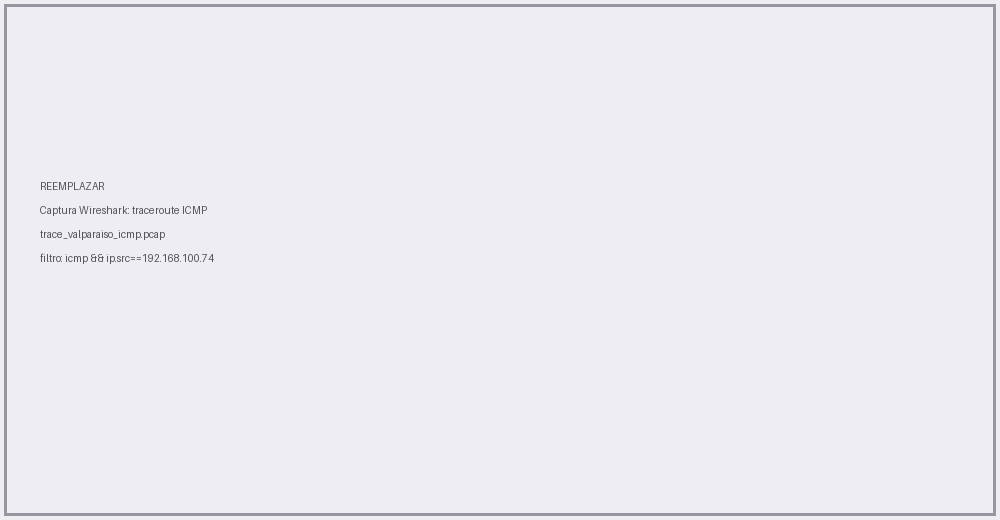
\includegraphics[width=0.9\textwidth]{figuras/wireshark_icmp.png}}
\caption{Traceroute ICMP a Valparaíso en Wireshark (\texttt{evidencia/pcap2/trace\_valparaiso\_icmp.pcap},
filtro \texttt{icmp \&\& ip.src==192.168.100.74}). Se aprecian los \emph{Echo Request} con TTL
creciente (1\dots11) y \texttt{seq} incremental, intercalados con los \emph{Time-Exceeded} de
cada router; el último (TTL 11) obtiene \emph{reply}, confirmando que ICMP completa la ruta.}
\end{figure}

\subsection{Nodo que filtra --- amenaza para el auditor}\label{sec:filtro}
El \emph{path discovery} no sólo revela qué nodos existen, sino también qué nodos \emph{se
ocultan} deliberadamente y mediante qué reglas. Desde la perspectiva de un auditor de seguridad
(o de un atacante), estos filtros son obstáculos que distorsionan el mapa de la red; identificar
la regla que los gobierna y la forma de sortearla es parte esencial del reconocimiento. En
nuestras mediciones se detectaron dos reglas de filtrado claramente distintas, una en el interior
de la red de Entel y otra en los propios destinos.

\paragraph{(1) Firewall \emph{stateful} que inyecta RST falsos (TCP-ACK).} En los tres destinos,
\texttt{tcp-ack} reporta ``llegar'' al destino en el salto 4 con un \texttt{[closed]} (RST). Es
\textbf{falso}: un \emph{middlebox} intercepta el ACK fuera de estado y responde con un RST
\textbf{falsificado} usando la IP del destino. La prueba está en el TTL:

\begin{table}[H]
\centering\small
\begin{tabular}{lcc}
\toprule
 & RST ``del destino'' (TCP-ACK, salto 4) & Echo-Reply genuino (ICMP, salto 11) \\
\midrule
\texttt{ip.src} & \ip{138.204.228.2} & \ip{138.204.228.2} \\
\textbf{\texttt{ip.ttl} de llegada} & \textbf{252} ($\approx$3 saltos) & \textbf{245} ($\approx$10 saltos) \\
\bottomrule
\end{tabular}
\caption{El RST llega con TTL 252 (origen a $\sim$3 saltos) mientras la respuesta real del
destino tiene TTL 245 (origen a $\sim$10 saltos): \emph{no provienen del mismo equipo}. El RST lo
genera un firewall \emph{stateful} de Entel ($\sim$salto 4, zona \ip{10.253.197.x}).}
\end{table}

\begin{figure}[H]
\centering
\fbox{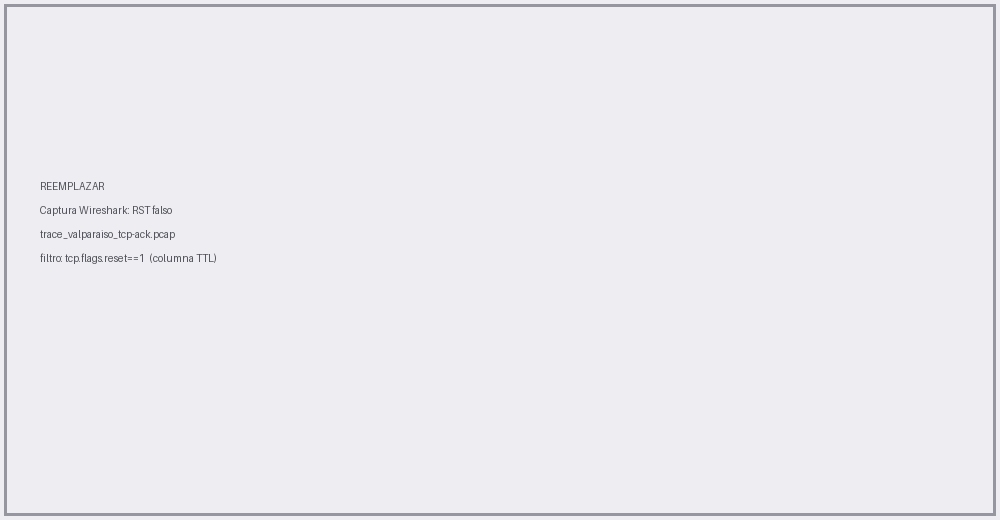
\includegraphics[width=0.9\textwidth]{figuras/wireshark_rst_falso.png}}
\caption{RST falsificado en \texttt{evidencia/pcap2/trace\_valparaiso\_tcp-ack.pcap}
(filtro \texttt{tcp.flags.reset==1}, columna TTL añadida). El paquete con origen
\ip{138.204.228.2} y flag ACK+RST llega con TTL 252, delatando su origen cercano.}
\end{figure}

El razonamiento forense que permite desenmascarar el engaño descansa por completo en el campo TTL
de la respuesta. Un paquete IP nace con un TTL inicial característico del sistema operativo que lo
emite (frecuentemente 64, 128 o 255) y se decrementa en cada salto. Si la respuesta genuina del
destino, situado a unos diez saltos, llega con TTL~245, su valor inicial fue 255 y recorrió
$255-245=10$ saltos, consistente con la distancia medida por ICMP. En cambio, el RST atribuido al
destino llega con TTL~252, lo que implica un origen a sólo $255-252=3$ saltos. Dos respuestas que
dicen provenir de la misma IP pero nacieron a distancias radicalmente distintas no pueden
proceder del mismo equipo: necesariamente una está falsificada. La conclusión es que un
\emph{middlebox} intermedio --un firewall \emph{stateful} dentro de la red de acceso de Entel,
en la zona \ip{10.253.197.x}-- intercepta el ACK y responde en nombre del destino.

\noindent\textbf{Regla:} descartar y responder con RST los segmentos ACK que no pertenecen a una
conexión establecida, comportamiento típico de defensa frente al \emph{ACK scan} (una técnica de
\emph{nmap} que usa ACKs sueltos para inferir reglas de firewall).
\textbf{Amenaza para el auditor:} quien confíe en \texttt{tcp-ack} obtendrá una topología
\emph{falsa} --el destino aparentando estar a cuatro saltos-- y un estado de puerto inventado,
lo que puede llevar a conclusiones erróneas sobre la cercanía y accesibilidad del objetivo.
\textbf{Cómo sortearla:} no fiarse de \texttt{tcp-ack} para la topología, emplear ICMP-Paris o SYN
real, y sobre todo \textbf{validar el TTL} de cada respuesta para detectar inyecciones de RST
como la descrita.

\paragraph{(2) Destinos que no responden a UDP.} \ip{138.204.228.2} y \ip{37.79.153.66}
\textbf{no responden} a UDP (no generan \emph{Port-Unreachable}), por lo que UDP/UDP-Paris nunca
completan; sí responden a \textbf{ICMP Echo}. \emph{Cómo saltarla:} cambiar a ICMP.

\subsection{\texttt{tracelb} --- traceroute con balanceo de carga}
El traceroute tradicional supone, implícitamente, que existe un único camino hacia el destino. En
la práctica, los operadores reparten el tráfico entre varios enlaces de igual coste (ECMP), por
lo que la ``ruta'' es en realidad un grafo de caminos paralelos. La utilidad \texttt{tracelb}
implementa un algoritmo de detección de rutas múltiples (MDA, \emph{Multipath Detection
Algorithm}) que, en lugar de enviar una sonda por salto, envía \emph{varias} con distintos
identificadores de flujo y observa cuándo flujos diferentes son desviados hacia próximos saltos
distintos, revelando así las ramas del balanceo. Se ejecutaron sus cinco modos
(\texttt{udp-dport}, \texttt{icmp-echo}, \texttt{udp-sport}, \texttt{tcp-sport},
\texttt{tcp-ack-sport}) por destino, que se diferencian en qué campo varían para generar los
distintos flujos.

\begin{table}[H]
\centering\small
\begin{tabular}{lccc}
\toprule
Destino & Traceroute (unión 6 métodos) & \texttt{tracelb} (unión 5 modos) & Unión total \\
\midrule
Valparaíso & 10 IPs & 10 IPs & 10 \\
La Habana & 17 IPs & 17 IPs & 17 \\
Rusia & 18 IPs & 18 IPs & \textbf{19} \\
\bottomrule
\end{tabular}
\caption{IPs únicas descubiertas. En volumen total \texttt{tracelb} es comparable a los 6
métodos de traceroute (en Rusia aporta 1 IP adicional).}
\end{table}

\noindent La ventaja de \texttt{tracelb} es revelar, \emph{en una sola medición}, varias IPs en
un mismo salto (ramas ECMP; p.ej. en La Habana \ip{200.0.16.21/25/29/62} coexistiendo). Envía
$\sim$6 sondas por salto, variando el identificador de flujo (\texttt{dport}, \texttt{sport} o
\texttt{icmp.checksum} según el modo). El modo \texttt{icmp-echo} es el que más nodos revela;
\texttt{tcp-ack-sport} se queda en 4 nodos por el mismo RST falso.

% ======================================================================
\section{Path Discovery con RIPE Atlas}
% ======================================================================
RIPE Atlas es una red de medición operada por el RIPE NCC compuesta por miles de sondas
distribuidas por el mundo que ejecutan, bajo demanda, mediciones de \emph{ping}, traceroute, DNS
o TLS. A diferencia de scamper, que mide desde un único punto, RIPE Atlas permite elegir el
\emph{origen} de la medición entre todas sus sondas, lo que habilita el experimento inverso de la
sección~5. El acceso se regula por un sistema de créditos: hospedar una sonda genera créditos que
luego se consumen al lanzar mediciones.

\subsection{Instalación de la sonda}
Se instaló una sonda por software (imagen \texttt{jamesits/ripe-atlas}) sobre Docker, en la misma
máquina de medición. El procedimiento sigue una lógica de clave pública: al arrancar, el
contenedor genera un par de claves y publica la pública; esa clave se registra en el formulario
de \url{https://atlas.ripe.net/apply/swprobe/} junto con la ubicación, y el \emph{backend} de
RIPE la autoriza para que la sonda pueda establecer el túnel de control. Durante el montaje se
enfrentaron y resolvieron varios obstáculos de permisos y de red (entre ellos, que un
\texttt{chown} recursivo sobre el proyecto rompía los permisos de los volúmenes del contenedor, y
que tras reiniciar la VM el contenedor debía relevantarse), todos documentados en el repositorio.
Superados, la sonda quedó \textbf{Connected}:
\begin{itemize}[nosep]
  \item \textbf{Probe ID: 1018349} --- \url{https://atlas.ripe.net/probes/1018349/}
  \item IPv4 \ip{186.10.176.77}, ASN 27651 (Entel), país CL.
\end{itemize}
Las mediciones se crearon vía la API REST seleccionando la sonda por ID (parámetros por defecto
de RIPE: \texttt{packets}=3, \texttt{size}=48, \texttt{paris}=0; UDP/TCP con puerto \ip{33435}).
Se optó por la API directa en lugar del cliente de línea de comandos porque éste exige por
defecto que la sonda posea la etiqueta \texttt{system-ipv4-works}, que una sonda recién conectada
y situada tras NAT (etiquetada \texttt{system-ipv4-rfc1918}) aún no ha obtenido; seleccionándola
explícitamente por su identificador se evita esa restricción. Un detalle que conviene anticipar
para leer correctamente las tablas es que, al ejecutarse la sonda dentro de un contenedor, su
primer salto es siempre la pasarela interna de Docker (\ip{172.17.0.1}); el resto de la ruta
coincide con la observada por scamper.

\subsection{Rutas e IPs con su AS, por protocolo}
\begin{table}[H]
\centering\footnotesize
\begin{tabular}{c|lll}
\toprule
HOP & ICMP (AS) & UDP (AS) & TCP (AS) \\
\midrule
1 & 172.17.0.1 (Docker) & 172.17.0.1 & 172.17.0.1 \\
2--7 & \multicolumn{3}{l}{192.168.100.1 $\to$ 100.83.128.1 $\to$ 10.253.197.9/.10 $\to$ 10.253.196.97 $\to$ 192.168.8.193 (todos priv.)} \\
8 & 45.68.16.129 (Entel) & 45.68.16.129 & * \\
9 & 10.100.154.1 & 10.100.154.1 & * \\
10 & 138.204.228.164 (AS61506) & 138.204.228.164 & * \\
11 & 138.204.228.162 (AS61506) & 138.204.228.162 & 138.204.228.162 \\
12 & \textbf{138.204.228.2 (AS61506)} & * & * \\
\bottomrule
\end{tabular}
\caption{RIPE --- Valparaíso. ICMP llega (12 saltos); UDP y TCP no. El salto 1 \ip{172.17.0.1}
es el \emph{gateway} Docker, porque la sonda corre containerizada.}
\end{table}

\begin{table}[H]
\centering\footnotesize
\begin{tabular}{c|lll}
\toprule
HOP & ICMP (AS) & UDP (AS) & TCP (AS) \\
\midrule
8 & 213.99.17.182 (AS12956, ES) & 213.99.17.182 & * \\
9 & 5.53.5.41 (AS12956) & 5.53.5.41 & * \\
10 & 213.140.35.86 (AS12956) & 213.140.35.86 & * \\
11 & 193.251.143.67 (AS5511, Orange) & 193.251.143.67 & * \\
14--16 & 200.0.16.62/21/29 (AS11960, ETECSA-IXP) & ídem & * \\
19/20 & \textbf{200.14.48.134 (AS27725)} & \textbf{200.14.48.134} & * \\
\bottomrule
\end{tabular}
\caption{RIPE --- La Habana (saltos 1--7 priv., omitidos). ICMP y UDP llegan; TCP no. Tránsito
internacional por Telxius (AS12956, España) y Orange (AS5511).}
\end{table}

\begin{table}[H]
\centering\footnotesize
\begin{tabular}{c|lll}
\toprule
HOP & ICMP (AS) & UDP (AS) & TCP (AS) \\
\midrule
8 & 213.99.17.182 (AS12956) & 213.99.17.182 & * \\
9 & 5.53.3.75 (AS12956) & 5.53.5.41 & 5.53.5.41 \\
11--15 & 195.2.x (AS1273, Vodafone) & 195.2.x & 195.2.x (parcial) \\
18 & 217.107.123.25 (AS12389) & 217.107.123.25 & * \\
19 & \textbf{37.79.153.66 (AS12389)} & * & * \\
\bottomrule
\end{tabular}
\caption{RIPE --- Rusia (saltos 1--7 priv., omitidos). Sólo ICMP llega. Tránsito por Telxius
(AS12956) y Vodafone (AS1273) hacia Rostelecom (AS12389).}
\end{table}

\subsection{Comparación de los tres protocolos}
\begin{table}[H]
\centering\small
\begin{tabular}{lccc c}
\toprule
Destino & ICMP & UDP & TCP & Más completo \\
\midrule
Valparaíso & sí (12) & no (11) & no (9) & \textbf{ICMP} \\
La Habana & sí (16) & sí (18) & no (7) & UDP/ICMP \\
Rusia & sí (17) & no (18) & no (12) & \textbf{ICMP} \\
\bottomrule
\end{tabular}
\caption{\textbf{ICMP} es el protocolo más indicado: único que completa la ruta en los tres
destinos, coherente con lo observado en scamper.}
\end{table}

La convergencia entre ambas herramientas es, en sí misma, un resultado valioso: scamper (desde el
\emph{host}) y RIPE Atlas (desde el contenedor) reconstruyen la \emph{misma} secuencia de sistemas
autónomos --Entel, luego Telxius (AS12956) en España, y de allí Orange (AS5511) hacia Cuba o
Vodafone (AS1273) hacia Rusia-- y coinciden en que ICMP es el protocolo que más infraestructura
revela. Esta reproducibilidad por dos vías independientes refuerza la confianza en el mapa
obtenido y muestra que las limitaciones observadas (destinos mudos ante UDP/TCP) son propiedades
de la red y no artefactos de una herramienta concreta. La principal diferencia metodológica es
que RIPE envía tres sondas por salto, lo que lo hace estadísticamente más robusto frente a
pérdidas puntuales.

\subsection{Análisis de tráfico (firmas de RIPE)}
\begin{table}[H]
\centering\footnotesize
\begin{tabularx}{\textwidth}{l l l X}
\toprule
Protocolo & L4 & Identificador & Observaciones \\
\midrule
ICMP & Echo t8 & \texttt{ident} fijo \textbf{36864} & \texttt{seq} incremental; 3 sondas/salto \\
UDP & UDP & \texttt{sport} fijo \textbf{20480}, \texttt{dport} incremental & payload mayor (\ip{ip.len}=76) \\
TCP & SYN & \texttt{sport} 20480, \texttt{dport} 33435 fijo & 3 sondas/salto \\
\bottomrule
\end{tabularx}
\caption{Firmas del software de sonda RIPE. Envía \textbf{3 sondas por salto} (vs 1 de scamper);
las constantes \ip{20480} (0x5000) y \ip{36864} (0x9000) son reconocibles. En el cable el origen
es \ip{192.168.100.74} (NAT del contenedor); la IP pública \ip{186.10.176.77} figura en el JSON.}
\end{table}

\begin{figure}[H]
\centering
\fbox{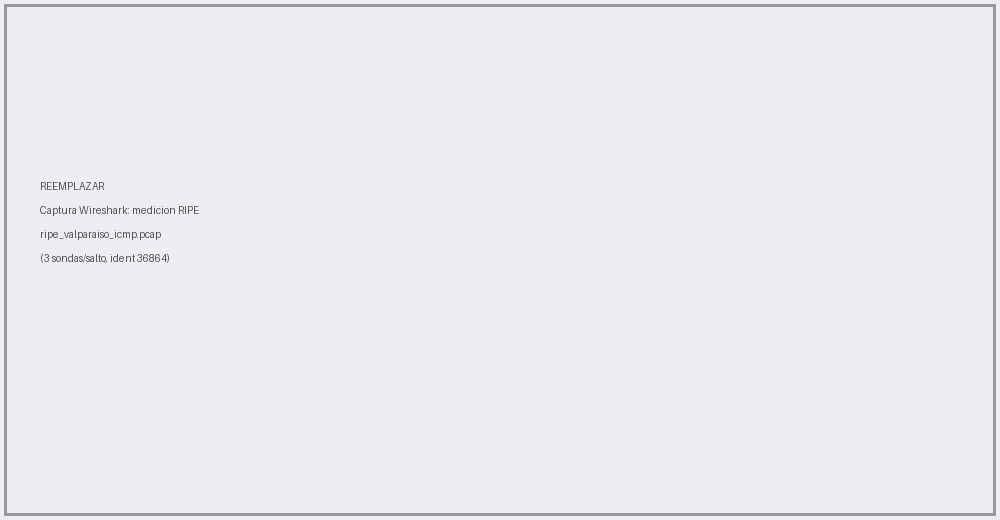
\includegraphics[width=0.9\textwidth]{figuras/wireshark_ripe.png}}
\caption{Tráfico de una medición RIPE (p.ej. ICMP) en Wireshark
(\texttt{evidencia\_ripe/pcap/ripe\_valparaiso\_icmp.pcap}). Se observan 3 sondas por TTL e
\texttt{ident} constante 36864.}
\end{figure}

\paragraph{Nodo que no responde.} \ip{138.204.228.2} y \ip{37.79.153.66} no responden a UDP ni
TCP-SYN pero sí a ICMP Echo (misma regla de filtrado que en scamper); se evade usando ICMP.

% ======================================================================
\section{Path way RIPE --- Ruta inversa}
% ======================================================================
Hasta aquí todas las mediciones nacían en nuestro acceso y viajaban hacia los destinos. Pero una
propiedad fundamental de Internet es que la ruta de ida no tiene por qué coincidir con la de
vuelta: cada sistema autónomo elige de forma independiente por dónde enviar su tráfico saliente,
siguiendo sus propias políticas BGP y acuerdos comerciales de tránsito y \emph{peering} (el
llamado encaminamiento \emph{hot-potato}, en que cada red entrega el tráfico a su vecino lo antes
posible). Medir en ambos sentidos permite, además, descubrir las \emph{dos} direcciones IP de
cada router --la interfaz de entrada y la de salida--, que el traceroute de un solo sentido nunca
muestra juntas. Para ello se aprovechó que los destinos son, a su vez, sondas RIPE: basta con
programar la medición \emph{desde} ellas hacia nuestra IP pública \ip{186.10.176.77}.

Se midió así la ruta inversa con los tres protocolos. La sonda de Valparaíso (31416) figuraba como
\emph{Abandoned} y no podía usarse como origen, por lo que se seleccionó la sonda \textbf{6652},
perteneciente al mismo sistema autónomo (AS61506, INSACOM) y a la misma zona geográfica, como
sustituta representativa. La Habana empleó la sonda 12734 y Rusia la 870, ambas originales del
enunciado.

\begin{table}[H]
\centering\footnotesize
\begin{tabular}{c|ll}
\toprule
HOP & IP IDA (AS) & IP VUELTA (AS) \\
\midrule
1 & 172.17.0.1 (Docker) & 138.204.230.193 (AS61506) \\
2 & 192.168.100.1 & 138.204.228.164 (AS61506) \\
3 & 100.83.128.1 & 10.100.163.1 (priv) \\
4 & 10.253.197.9 & 10.100.154.2 (priv) \\
5 & 10.253.197.10 & \textbf{45.68.17.13} (priv) \\
6 & 10.253.196.97 & \textbf{192.168.8.194} (priv) \\
7--9 & 192.168.8.193 / 45.68.16.129 / 10.100.154.1 & * \\
10--12 & 138.204.228.164/.162/.2 (AS61506) & --- \\
\bottomrule
\end{tabular}
\caption{Tabla 2 --- Valparaíso (ICMP ida / vuelta). Aparecen \textbf{interfaces espejo}:
\ip{45.68.16.129}$\leftrightarrow$\ip{45.68.17.13}, \ip{192.168.8.193}$\leftrightarrow$\ip{192.168.8.194},
\ip{10.100.154.1}$\leftrightarrow$\ip{10.100.154.2}, es decir las dos IPs de un mismo router,
objetivo del \emph{path way} bidireccional.}
\end{table}

\begin{table}[H]
\centering\footnotesize
\begin{tabular}{c|ll}
\toprule
HOP & IP IDA (AS) & IP VUELTA (AS) \\
\midrule
7 & 192.168.9.133 (priv) & 200.0.16.20 (AS11960) \\
8 & 213.99.17.182 (AS12956, ES) & 89.221.37.138 (\textbf{AS6762}, TI Sparkle, IT) \\
9 & 5.53.5.41 (AS12956) & 89.221.41.155 (AS6762) \\
11 & 193.251.143.67 (AS5511, Orange) & 181.78.91.246 (\textbf{AS52468}, UFINET, PA) \\
12 & * & 190.211.160.5 (AS52468) \\
19/20 & 200.14.48.178/.134 (AS27725) & --- \\
\bottomrule
\end{tabular}
\caption{Tabla 2 --- La Habana (ICMP). \textbf{0 IPs comunes.} IDA por Telxius+Orange; VUELTA por
Telecom Italia Sparkle (AS6762) + UFINET Panamá (AS52468) + Level3: ruteo totalmente asimétrico.}
\end{table}

\begin{table}[H]
\centering\footnotesize
\begin{tabular}{c|ll}
\toprule
HOP & IP IDA (AS) & IP VUELTA (AS) \\
\midrule
2 & 192.168.100.1 & 80.71.208.90 (AS12389, Rostelecom) \\
3 & 100.83.128.1 & 87.226.151.158 (AS12389) \\
7 & 192.168.9.133 & 193.251.133.3 (\textbf{AS5511}, Orange) \\
9 & 5.53.3.75 (AS12956) & 200.189.207.14 (\textbf{AS3549}, Level3) \\
10 & 94.142.118.184 (AS12956) & 8.243.188.94 (\textbf{AS3356}, Level3) \\
11--15 & 195.2.x (AS1273, Vodafone) & * \\
18/19 & 217.107.123.25 / 37.79.153.66 (AS12389) & --- \\
\bottomrule
\end{tabular}
\caption{Tabla 2 --- Rusia (ICMP). \textbf{0 IPs comunes.} IDA por Vodafone (AS1273); VUELTA por
Level3 (AS3356/3549). Asimetría total también a nivel de AS.}
\end{table}

\begin{table}[H]
\centering\small
\begin{tabular}{lccc}
\toprule
Destino & IPs comunes ida/vuelta & ¿Misma ruta? & ¿Misma cantidad de IPs? \\
\midrule
Valparaíso & 1 (interfaces espejo) & No & No (IDA 9--12 vs VUELTA 6--7) \\
La Habana & 0 & No, asimétrica & No (IDA 16--18 vs VUELTA 11--12) \\
Rusia & 0 & No, asimétrica & No (IDA 17--18 vs VUELTA 7--9) \\
\bottomrule
\end{tabular}
\caption{Resumen ida vs vuelta. El ruteo es \textbf{asimétrico} en los tres casos: ni la ruta ni
el número de IPs coinciden, y a nivel de AS los proveedores de tránsito difieren por sentido.}
\end{table}

Los resultados confirman de forma contundente la asimetría anticipada, pero en dos grados
distintos que conviene interpretar. En Valparaíso la asimetría es \emph{de interfaz}: ida y
vuelta transcurren por la misma región de la red de Entel/INSACOM, pero cada router aparece con
una IP distinta en cada sentido --\ip{45.68.16.129} de ida frente a \ip{45.68.17.13} de vuelta,
\ip{192.168.8.193} frente a \ip{192.168.8.194}, \ip{10.100.154.1} frente a \ip{10.100.154.2}--.
Estos pares son las dos caras de un mismo equipo, y sólo midiendo en ambos sentidos se les puede
emparejar; es, precisamente, el objetivo del \emph{path way} bidireccional. En La Habana y Rusia,
en cambio, la asimetría es \emph{de proveedor}: no comparten ni una sola IP (cero IPs comunes) y
el tránsito internacional cambia por completo de operador según el sentido. El tráfico hacia Cuba
sale por Telxius (España) y Orange, pero regresa por Telecom Italia Sparkle, UFINET (Panamá) y
Level3; el de Rusia va por Vodafone y vuelve por Level3. Esta divergencia no es un error de
medición sino el reflejo directo de las políticas de ruteo: la red de destino entrega su tráfico
de retorno al tránsito que le resulta más conveniente, que rara vez es el espejo del de ida. Para
un auditor, la lección es doble: un único traceroute ofrece una visión \emph{parcial y sesgada} de
la conectividad, y la combinación de ambos sentidos casi duplica la cantidad de interfaces y
operadores observados.

% ======================================================================
\section{Public Path --- Grafos en NDEx}
% ======================================================================
El paso final consiste en sintetizar el conocimiento disperso en las tablas anteriores en una
representación visual e interoperable. Un grafo es la estructura natural para ello: los routers
son nodos y los saltos observados son aristas. Al unir en un mismo grafo la ruta de ida y la de
vuelta, los nodos que comparten dirección IP se fusionan automáticamente, de modo que el grafo
expone de un vistazo tanto los puntos comunes como las divergencias y las interfaces espejo
discutidas en la sección anterior. Se eligió NDEx (\emph{Network Data Exchange}) como repositorio
por ser una plataforma abierta y citable que asigna a cada red un identificador persistente
(UUID), lo que facilita la verificación independiente del resultado.

Por cada destino se tomó la ruta más completa (ida + vuelta) y se generó un grafo dirigido
(nodos = IPs con atributo AS; aristas = saltos con atributo \texttt{direction}), publicado en
\url{https://www.ndexbio.org/}. Siguiendo la consigna, la descripción de cada grafo incluye los
dos identificadores de medición RIPE (ida y vuelta) que lo originaron, de modo que cualquiera
pueda reconstruirlo desde los datos crudos.

\begin{table}[H]
\centering\footnotesize
\begin{tabularx}{\textwidth}{l X cc}
\toprule
Destino & UUID & ID ida & ID vuelta \\
\midrule
Valparaíso & \texttt{0acc00aa-ccbe-11f1-be0a-005056ae3c32} & 225408742 & 225423796 \\
La Habana & \texttt{0b0957cd-ccbe-11f1-be0a-005056ae3c32} & 225411975 & 225424159 \\
Rusia & \texttt{0b48f7e0-ccbe-11f1-be0a-005056ae3c32} & 225412819 & 225428926 \\
\bottomrule
\end{tabularx}
\caption{Grafos publicados (3 UUID) y las dos mediciones RIPE usadas en cada uno. Visor:
\texttt{https://www.ndexbio.org/viewer/networks/<UUID>}. Tamaños: Valparaíso 17 nodos, La Habana
28 nodos, Rusia 25 nodos.}
\end{table}

\begin{figure}[H]
\centering
\fbox{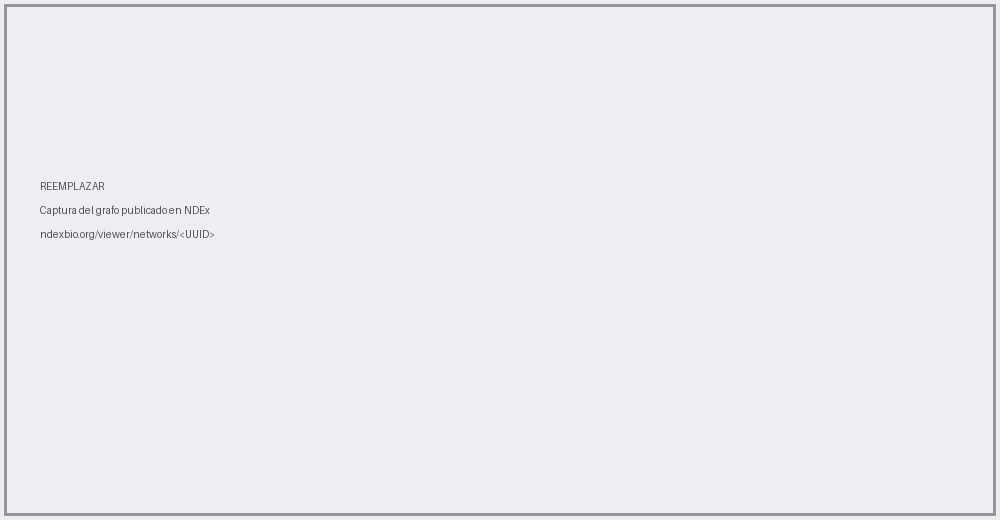
\includegraphics[width=0.8\textwidth]{figuras/ndex_grafo.png}}
\caption{Ejemplo de grafo de ruta publicado en NDEx (ida+vuelta). Los nodos con misma IP se
fusionan, exponiendo interfaces espejo y la asimetría de ruteo.}
\end{figure}

% ======================================================================
\section{Conclusiones}
% ======================================================================
El recorrido completo --desde la identificación del punto de observación hasta la publicación de
los grafos-- permitió caracterizar con detalle la infraestructura que conecta un acceso
residencial chileno con tres puntos representativos del planeta, y contrastar dos metodologías de
medición que resultaron mutuamente confirmatorias. Los principales hallazgos se resumen así:

\begin{itemize}[nosep]
  \item La conexión BAF pertenece a \textbf{Entel (AS27651)}, prefijo anunciado \ip{186.10.176.0/24}.
  \item En ambas herramientas, \textbf{ICMP/ICMP-Paris} es el método más completo para descubrir
  la ruta; UDP y TCP fallan ante destinos que filtran esos protocolos.
  \item Se identificó un \textbf{firewall \emph{stateful} de Entel} que inyecta RST falsos ante
  TCP-ACK (detectado por incoherencia de TTL: 252 vs 245) --- una trampa para un auditor.
  \item El \textbf{ruteo es asimétrico}: ida y vuelta usan rutas e incluso proveedores de tránsito
  distintos (Cuba: Telxius/Orange vs Telecom Italia/UFINET/Level3; Rusia: Vodafone vs Level3).
  \item Medir en ambos sentidos reveló \textbf{interfaces espejo} de los routers, integradas en
  los tres grafos publicados en NDEx.
\end{itemize}

\noindent En términos de la ``amenaza para el auditor'' que atraviesa todo el trabajo, la
conclusión práctica es que ninguna técnica de sondeo es, por sí sola, confiable: los filtros de
red producen silencios (destinos mudos ante UDP) y, peor aún, mentiras activas (RST falsificados
que fingen un destino cercano). Un reconocimiento riguroso exige, por tanto, combinar varios
métodos y protocolos, medir en ambos sentidos y validar la coherencia interna de las respuestas
--por ejemplo mediante el TTL-- antes de dar por buena la topología inferida. El valor del
\emph{path discovery} no reside en una sola traza, sino en la triangulación de muchas.

\appendix
\section{Evidencia y reproducibilidad}
\begin{itemize}[nosep]
  \item \textbf{Scamper:} 33 mediciones (\texttt{.warts}, \texttt{.txt}, \texttt{.pcap}) en
  \texttt{evidencia/}.
  \item \textbf{RIPE:} 9 mediciones de ida + 9 de vuelta (IDs, JSON, pcap) en
  \texttt{evidencia\_ripe/}; todas verificables en \texttt{atlas.ripe.net/measurements/<ID>/}.
  \item \textbf{Scripts:} \texttt{run\_scamper\_p1.sh}, \texttt{run\_ripe\_p2.sh},
  \texttt{run\_ripe\_p4.sh}, \texttt{build\_graphs.py}, entre otros.
  \item Todos los enlaces (mediciones RIPE, grafos NDEx) están en \texttt{informe/LINKS.md}.
\end{itemize}

\end{document}
